% !TeX program = xelatex
\documentclass[UTF8,fontset=fandol,zihao=-4,a4paper,oneside,openany]{ctexbook}
\usepackage{fontspec}
\usepackage[margin=1in,headheight=16pt]{geometry}
\usepackage{amsmath,amssymb}
\usepackage{enumitem}
\setlist{nosep,leftmargin=2em,topsep=4pt}
\usepackage{booktabs,longtable,array}
\usepackage[table]{xcolor}
\usepackage[most]{tcolorbox}
\usepackage{fvextra}
\usepackage{tikz}
\usetikzlibrary{positioning,arrows.meta,fit,calc}
\usepackage{fancyhdr}
\usepackage{needspace}
\PassOptionsToPackage{obeyspaces}{url}
\usepackage{xurl}
\usepackage{hyperref}
\hypersetup{unicode=true,hypertexnames=false,colorlinks=true,linkcolor=blue!45!black,
 urlcolor=blue!55!black,bookmarksnumbered=true,
 pdftitle={Bumi 机器人综合使用手册},
 pdfsubject={硬件、日常使用与 SDK 开发}}
\urlstyle{tt}
\setmonofont{Latin Modern Mono}[Scale=MatchLowercase,BoldFont=lmmonolt10-bold.otf]
\setlength{\emergencystretch}{2em}
\setlength{\parskip}{3pt}
\setlength{\LTpre}{6pt}
\setlength{\LTpost}{8pt}
\renewcommand{\arraystretch}{1.25}
\setcounter{tocdepth}{1}
\setcounter{secnumdepth}{1}
\newcommand{\handbookchaptertitle}{}
\newcommand{\setchapterheader}[1]{\gdef\handbookchaptertitle{#1}}
\newcommand{\handbookpagestyle}{%
  \fancyhf{}%
  \fancyhead[L]{\small\kaishu\handbookchaptertitle}%
  \fancyhead[R]{\small\kaishu\thepage}%
  \renewcommand{\headrulewidth}{0.4pt}%
  \renewcommand{\footrulewidth}{0pt}%
}
\pagestyle{fancy}
\handbookpagestyle
\fancypagestyle{plain}{\handbookpagestyle}
\DeclareRobustCommand{\code}[1]{{\small\nolinkurl{#1}}}
\newcommand{\stepref}[1]{第\,#1\,步（第\,\pageref{step:#1}\,页）}
\tcbset{handbook/.style={enhanced,breakable,boxrule=0.4pt,arc=3pt,
 left=6pt,right=6pt,top=5pt,bottom=5pt,fonttitle=\bfseries,
 before skip=8pt,after skip=8pt}}
\newtcolorbox{intro}{handbook,colback=green!5,colframe=green!50!black,
 colbacktitle=green!50!black,coltitle=white,title=本章内容}
\newtcolorbox{remark}[1]{handbook,colback=yellow!5,colframe=yellow!50!black,
 colbacktitle=yellow!50!black,coltitle=white,title={#1}}
\newtcolorbox{concept}[1]{handbook,colback=cyan!3,colframe=cyan!50!black,
 colbacktitle=cyan!50!black,coltitle=white,title={#1}}
\newtcolorbox{expected}{handbook,colback=blue!4,colframe=blue!50!black,
 colbacktitle=blue!50!black,coltitle=white,title=预期结果}
\newtcolorbox{faq}[1]{handbook,colback=yellow!4,colframe=yellow!45!black,
 colbacktitle=yellow!45!black,coltitle=white,title={#1}}
\DefineVerbatimEnvironment{command}{Verbatim}{fontsize=\small,
 baselinestretch=1,frame=single,framesep=2mm,rulecolor=\color{black!65},
 samepage=true,breaklines=true,breakanywhere=true,tabsize=4,showspaces=false,showtabs=false}
\newcolumntype{P}[1]{>{\raggedright\arraybackslash}p{#1}}

\usepackage{fontawesome5}
\usepackage{graphicx}
\usepackage{float}
\usepackage{caption}
\captionsetup{font=small,labelfont=bf}
\newcommand{\official}{https://noetixrobotics.feishu.cn/docx/As2adPO27odPBfxQw1ucK6N4nNe}
\newcommand{\officiallink}[2]{\href{\official\##1}{#2}}
\newcommand{\diagram}[2]{\begin{figure}[H]\centering #2\caption{#1}\end{figure}}
\tikzset{box/.style={draw=cyan!50!black,fill=cyan!4,rounded corners,align=center,minimum height=11mm,text width=36mm,font=\small},flow/.style={-{Stealth},thick,draw=black!65}}

\begin{document}
\begin{titlepage}
\centering
\vspace*{0.10\textheight}
{\Huge\bfseries Bumi 机器人\par}
\vspace{0.55cm}
{\huge\bfseries 综合使用手册\par}
\vspace{1.0cm}
{\large 祁果\par}
\vspace{0.35cm}
{\small\faGithub\ \href{https://github.com/77-GGG/bumi-handbooks}{\texttt{77-GGG/bumi-handbooks}}\par}
\vspace{0.5cm}
{\small\today\par}
\vspace{1.2cm}
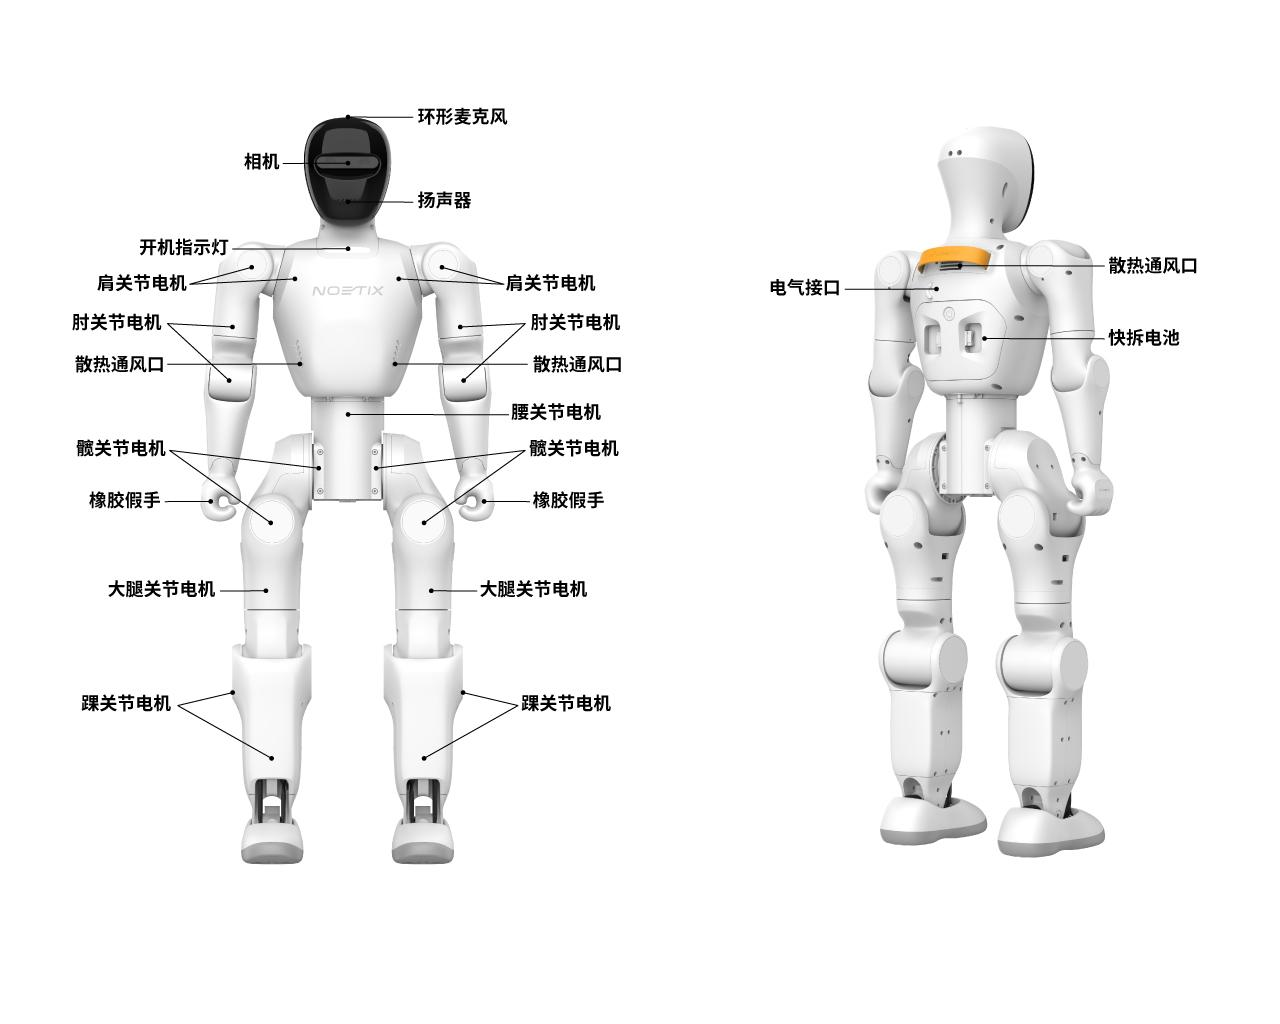
\includegraphics[width=0.62\linewidth]{images/bumi-components.jpg}
\vfill
\end{titlepage}
\frontmatter
\chapter*{前言}
\setchapterheader{前言}
\addcontentsline{toc}{chapter}{前言}
拿到一台机器人后，我们通常会先遇到三件事：认识它的部件，把它开起来，再让自己的程序与它通信。这本手册按这个顺序展开，先介绍硬件和日常操作，再说明开发环境，最后进入运动、音频和相机接口。

第一次使用 Bumi，可以从前两章开始，完成安装电池、连接 APP、起身和收纳。准备开发程序时，接着阅读第三至第五章，熟悉终端、Conda、网络和编译流程。调用出厂动作主要使用 HighController；部署自己的关节控制或运动策略，则使用 LowController。音视频接口和相机采集各自成章，便于按任务查阅。

命令需要在 Ubuntu 终端中执行。代码框中的路径和地址都对应具体用途：\code{~/noetix_sdk_bumi} 是本书示例使用的 SDK 根目录，\code{bumi_deploy} 是编译和运行共用的 Conda 环境，\code{192.168.55.102} 是运控板的默认地址。理解这些名字之后，再按自己的目录和网络填写命令，会更容易找到问题。

本文按\href{https://noetixrobotics.feishu.cn/docx/As2adPO27odPBfxQw1ucK6N4nNe}{《Bumi 综合使用文档》}重新编排，并结合其链接的编译环境、音视频说明及项目内 SDK 3.1.0 核对示例。正文中的表格用于查参数，命令框用于操作，提示框解释动作发生的条件。附录集中列出控制命令、工作模式、关节范围和视频入口。

\clearpage\setchapterheader{目录}
\tableofcontents
\mainmatter
\chapter{认识 Bumi}
\setchapterheader{第\thechapter 章\quad 认识 Bumi}

\begin{intro}
认识机器人的自由度、版本、接口和机载计算机，查阅相机、电池与充电器参数。
\end{intro}
\section{部件与自由度}
Bumi 全身共有 21 个自由度。这里的自由度可以理解为一个独立控制的关节转动方向。单臂有 4 个，单腿有 6 个，腰部有 1 个，因此总数为 $2\times4+2\times6+1=21$。
\begin{itemize}
\item 手臂：肩关节 pitch、肩关节 roll、上臂 yaw、肘关节 pitch。
\item 腿部：髋关节 pitch、髋关节 roll、大腿 yaw、膝关节 pitch、踝关节 pitch、踝关节 roll。
\item 腰部：腰关节 yaw。
\end{itemize}
pitch、roll 和 yaw 分别表示俯仰、横滚和偏航。具体关节的正方向要结合模型坐标系阅读，电机编号、名称和范围见附录\ref{app:joints}。
\begin{figure}[H]
\centering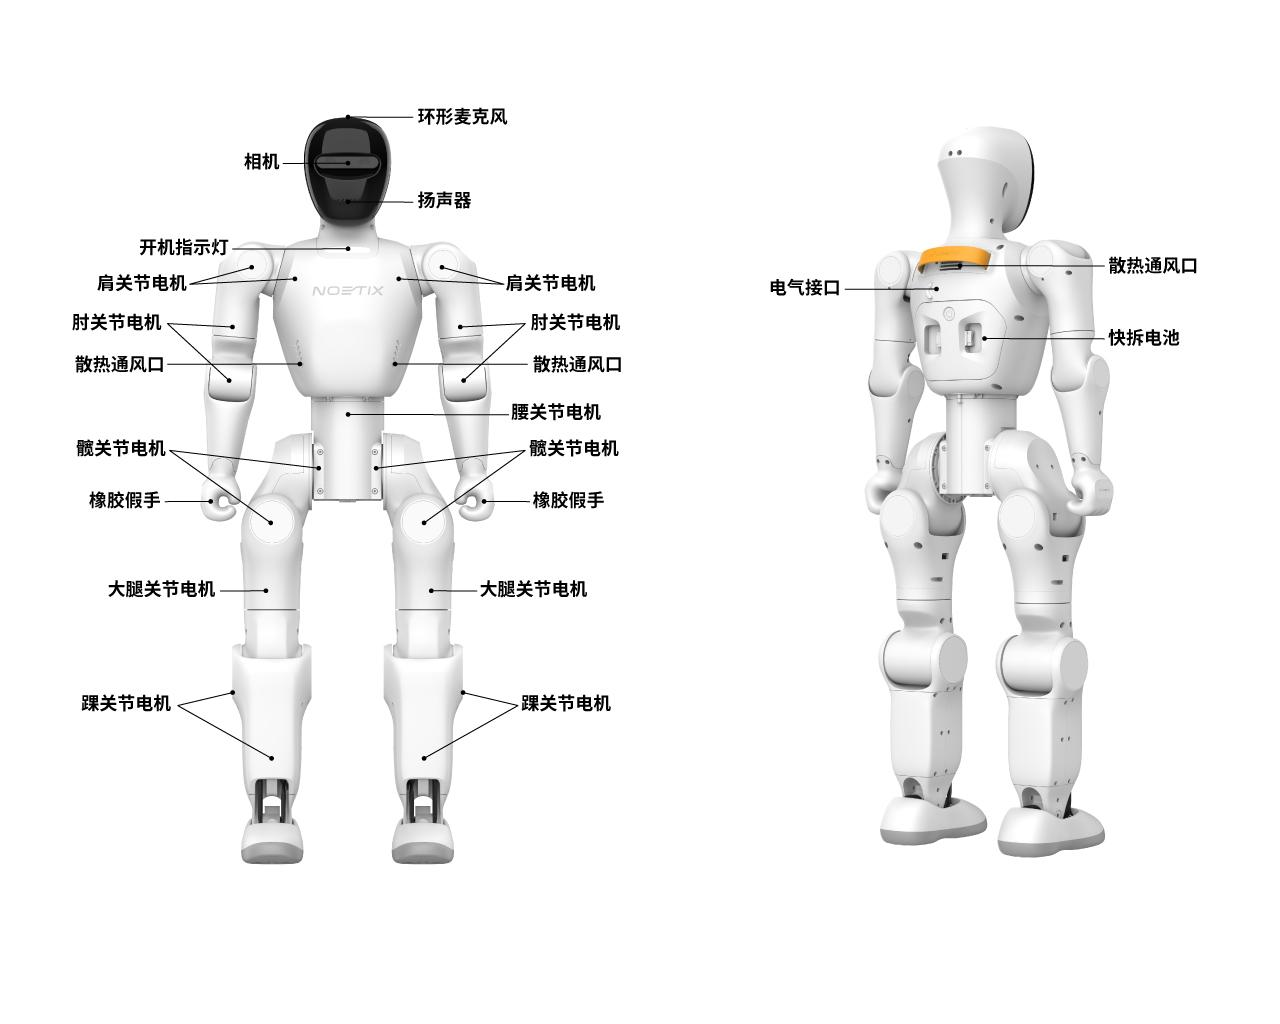
\includegraphics[width=0.72\linewidth]{images/bumi-components.jpg}
\caption{Bumi 部件示意图}
\end{figure}
\section{整机参数与版本}

\begingroup\small\renewcommand{\arraystretch}{1.15}
\begin{longtable}{@{}P{0.32\linewidth}P{0.61\linewidth}@{}}
\toprule
\textbf{项目} & \textbf{参数} \\
\midrule\endhead
站立尺寸（高、宽、厚） & 约 98 cm $\times$ 35 cm $\times$ 20 cm \\
带电池重量 & 约 17 kg \\
总自由度 & 21；单臂 4、单腿 6、腰部 1 \\
关节通信 & EtherCAT 与 CAN FD \\
整机规格表中的最大关节扭矩 & 70 N·m \\
大腿与小腿长度 & 合计约 513 mm \\
手臂长度 & 约 312 mm \\
供电 & 快拆锂电池；标称续航 2--3 小时 \\
感知与交互 & IMU、相机、麦克风阵列、扬声器、APP 与 OTA \\
\bottomrule\end{longtable}\endgroup

官方外形尺寸图标注的整机高度为 988 mm，宽度为 350.46 mm，侧向厚度为 203.20 mm。整机概览采用取整尺寸；安装与结构设计可在\officiallink{J7iRd3pqzo6ICqxdHyHcfakQnff}{外观件尺寸图}中查看完整尺寸标注。关节控制使用附录中的逐关节参数。

\begingroup\small\renewcommand{\arraystretch}{1.15}
\begin{longtable}{@{}P{0.22\linewidth}P{0.27\linewidth}P{0.42\linewidth}@{}}
\toprule
\textbf{项目} & \textbf{标准版} & \textbf{教育版} \\
\midrule\endhead
基础算力 & 6 TOPS & 6 TOPS，部分型号另配 67 / 117 TOPS 算力板 \\
算力模块 & 无独立 Jetson 算力板 & Jetson Orin Nano Super / NX；部分型号无算力板 \\
相机 & \code{DC_V93} & RealSense D435i；EDU\_Air 除外 \\
图传 & 通过 APP 使用 & 开发时可在算力板访问相机硬件 \\
HighController & 支持 & 支持 \\
LowController & 未开放 & 支持 \\
\bottomrule\end{longtable}\endgroup

\section{背部电气接口}
背部提供 1 个 RJ45 千兆以太网口、2 个 USB 3.0 接口和 1 个 HDMI 接口。RJ45 采用 1000BASE-T。配有算力板的版本，背部接口连接算力板；未配算力板的版本，接口连接运控板。接线位置见\officiallink{doxcnqSG6s08595TTZSMDbgjqRb}{官方电气接口图}。
\section{机载计算机}
机器人内部的运控板负责运动控制。教育版中的 Jetson 算力板用于运行用户程序，两者通过网络通信。

\begingroup\small\renewcommand{\arraystretch}{1.15}
\begin{longtable}{@{}P{0.17\linewidth}P{0.23\linewidth}P{0.25\linewidth}P{0.25\linewidth}@{}}
\toprule
\textbf{项目} & \textbf{运控板} & \textbf{算力板 Nano Super} & \textbf{算力板 NX} \\
\midrule\endhead
平台 & RK3576 & Jetson Orin Nano Super & Jetson Orin NX \\
默认 IP & \code{192.168.55.102} & \code{192.168.55.101} & \code{192.168.55.101} \\
算力 & 6 TOPS & 67 TOPS & 117 TOPS \\
主频 & 2.4 GHz & 1.7 GHz & 2.0 GHz \\
内存与存储 & 8 + 64 GB & 8 + 128 GB & 16 + 128 GB \\
用户登录 & 通过 SDK 接口访问功能 & 用户 \code{noetix} & 用户 \code{noetix} \\
\bottomrule\end{longtable}\endgroup

算力板出厂账户为 \code{noetix}，初始密码为 \code{bumi}。开发时登录算力板，运动命令通过 SDK 发给运控板。
\section{相机}
标准版使用 DC\_V93 USB 摄像模组，最高有效像素为 $2592\times1944$。教育版的 D435i 使用方法见第\ref{chap:camera}章。

\begingroup\small\renewcommand{\arraystretch}{1.15}
\begin{longtable}{@{}P{0.29\linewidth}P{0.63\linewidth}@{}}
\toprule
\textbf{DC\_V93 项目} & \textbf{参数} \\
\midrule\endhead
感光尺寸与像素尺寸 & 1/4 英寸；$1.4\,\mu$m $\times$ $1.4\,\mu$m \\
图像格式 & MJPEG；YUV2（YUYV） \\
接口 & USB 2.0 High Speed \\
对焦 & 固定 / AF \\
中心清晰度 & 800 LW/PH（Center） \\
信噪比与动态范围 & 36 dB；71.6 dB \\
灵敏度与最低照度 & 1.4 V/lux-sec @ 550 nm；0.5 lux \\
自动控制 & 支持自动曝光、自动白平衡、自动增益 \\
镜头 & 焦距 6.78 mm；光圈 F2.4；对角视场角 32.6° \\
可调参数 & 亮度、对比度、饱和度、色调、清晰度、伽马、白平衡、逆光对比、曝光度 \\
\bottomrule\end{longtable}\endgroup

\begingroup\small\renewcommand{\arraystretch}{1.15}
\begin{longtable}{@{}P{0.35\linewidth}P{0.26\linewidth}P{0.28\linewidth}@{}}
\toprule
\textbf{分辨率} & \textbf{MJPEG 帧率} & \textbf{YUV 帧率} \\
\midrule\endhead
$2592\times1944$ & 30 fps & 2 fps \\
$1920\times1080$ & 30 fps & 5 fps \\
$1280\times720$ & 30 fps & 8 fps \\
$848\times480$ & 30 fps & 20 fps \\
$640\times480$ & 30 fps & 30 fps \\
\bottomrule\end{longtable}\endgroup

\section{电池与充电器}

\begingroup\small\renewcommand{\arraystretch}{1.15}
\begin{longtable}{@{}P{0.3\linewidth}P{0.62\linewidth}@{}}
\toprule
\textbf{电池项目} & \textbf{参数} \\
\midrule\endhead
生产商 & 深圳格瑞普 \\
型号 & \code{GRP6752097-13S1P} \\
容量 & 5100 mAh \\
标称电压 & 48 V \\
重量 & 1360 g \\
\bottomrule\end{longtable}\endgroup

\begingroup\small\renewcommand{\arraystretch}{1.15}
\begin{longtable}{@{}P{0.3\linewidth}P{0.62\linewidth}@{}}
\toprule
\textbf{充电器项目} & \textbf{参数} \\
\midrule\endhead
型号 & TA300 Robot 智能充电器 \\
输入 & 100--240 V AC；50/60 Hz；4.5 A \\
支持电池 & LiPo / LiFe / LiHV；13S--16S \\
输出 & 35--72 V DC；7.5 A；最大 350 W \\
尺寸 & $172\times97\times46$ mm \\
重量 & $510\pm10$ g \\
工作模式 & 充电 \\
\bottomrule\end{longtable}\endgroup

\chapter{开机、连接与充电}
\setchapterheader{第\thechapter 章\quad 开机、连接与充电}

\begin{intro}
完成电池安装、启动、APP 连接、动作操作和关机充电，了解机器人运动所需的场地与摆放条件。
\end{intro}
\section{准备场地}
选择平整、干燥、防滑的地面。起身和收纳时，周围留出约 $3\times3$ m 的空间；舞蹈和移动时，根据动作幅度继续扩大活动区域，让人员、线缆和物品处于运动范围外。

雨水、潮湿和水雾会影响电气部件。松软地面、台阶、凹凸路面以及超过 20° 的坡面也会改变支撑条件。第一次使用从平整地面开始，开发调试全程使用吊架。
\section{安装电池与启动}
\begin{enumerate}
\item 从包装中取出机器人，放成稳定坐姿。
\item 将电池插入背部电池仓，确认卡扣锁定。
\item 短按电源键，看到指示灯后再长按，直到出现流水灯，等待启动完成。
\item 按操作要求将机器人面朝上平放，双腿伸直，手臂自然放在腰部两侧，给关节回零留出空间。
\end{enumerate}
\begin{remark}{起身前的姿态}
“一键起身”从面朝上平躺的姿态开始。保持身体平放、四肢自然展开，关节处于可活动范围内。使用“辅助起身”时，按该功能的要求扶持机器人站立，再进行使能。
\end{remark}
\section{使用 Noetix Run}
在手机上安装 Noetix Run。iPhone 可通过\href{https://apps.apple.com/cn/app/noetix-run/id6751874215}{App Store 页面}安装；Android 下载二维码位于\officiallink{doxcn9WNtopSlikdBsw6SrXBVJ7}{官方 APP 章节}。打开 APP 后，按界面完成激活、绑定和设备连接，再使用起身、移动、基本动作、示教、舞蹈、动作库、图传和语音功能。

手机与机器人之间使用蓝牙和 Wi-Fi 通信，官方连接图同时给出了这两条链路。配网时按 APP 提示选择网络，保持手机和机器人的连接条件。
\diagram{手机与机器人的连接关系}{
\begin{tikzpicture}[node distance=18mm]
\node[box] (phone) {手机\\Noetix Run};
\node[box,right=42mm of phone] (robot) {Bumi};
\node[box,above right=15mm and 3mm of phone] (wifi) {Wi-Fi 网络};
\draw[flow,<->] (phone)--node[below,font=\small]{蓝牙}(robot);
\draw[flow,<->] (phone)--(wifi);
\draw[flow,<->] (robot)--(wifi);
\end{tikzpicture}}
\begin{remark}{保留蓝牙配对记录}
完成连接后保留手机系统中的设备配对记录。官方手册指出，使用“忽略设备”会清除蓝牙记录，之后可能需要售后协助恢复连接。
\end{remark}
APP 的逐项操作见\href{http://app-file.noetixrobotics.com/page/appUseCn.html}{Noetix Run 使用说明}。附录\ref{app:resources}按操作顺序列出了官方视频入口。
\section{移动与动作切换}
先完成起身并确认站稳，再使用移动或动作功能。每次切换后观察机器人当前状态，等前一个动作完成再进行下一项操作。快速连续切换会叠加身体惯性。

机器人行走时，控制器会继续输出关节力矩。需要搬动机器人时，先停止移动，再按收纳与关机流程操作。关节运动时，让手、衣物和线缆离开关节间隙。
\section{收纳与关机}
\begin{enumerate}
\item 在 APP 中执行“一键收纳”，等待机器人进入稳定坐姿。
\item 长按电源键关机，确认设备停止工作。
\item 按下电池卡扣，取出电池。
\end{enumerate}
\section{充电}
将取出的电池放到配套充电底座并接好适配器，再把充电器接入交流电源。官方操作示例使用 220 V 插座，充电器输入范围见上一章。

充电过程中指示灯闪烁，充满后无指示。充电完成后断开充电器，妥善保存电池和线缆；下次使用时重新装入机器人。

\chapter{开发前的基础知识}
\setchapterheader{第\thechapter 章\quad 开发前的基础知识}

\begin{intro}
理解终端、工作目录、Python 扩展、虚拟环境和控制周期，为后面的编译与接口调用建立共同语境。
\end{intro}
\section{终端与工作目录}
终端把输入的命令交给 Shell 执行。开发时经常同时打开几个终端，每个终端都有自己的工作目录和环境。进入一个终端后，先看当前在哪里，再选择项目环境：
\par\noindent\begin{minipage}{\linewidth}
\begin{command}
pwd
ls
cd ~/noetix_sdk_bumi
conda activate bumi_deploy
\end{command}
\end{minipage}\par

\code{pwd} 显示当前位置，\code{ls} 列出文件，\code{cd} 切换目录。波浪号表示当前用户的主目录。\code{./build}、\code{config/dds.xml} 等相对路径从当前工作目录出发，因此本书的 SDK 命令都从项目根目录执行。

长命令末尾的反斜杠表示续行，下一行仍属于同一条命令。命令后的参数用于指定选项，例如 \code{--parallel 2} 让构建工具同时使用两个任务。
\section{Python、C++ 与 SDK}
C++ 源文件先经编译和链接，生成可执行程序或共享库。Python 脚本由解释器执行；当它导入 \code{highcontrol_py} 时，实际加载的是 C++ 经 pybind11 封装的扩展模块。

这意味着 Python 示例也需要先编译 SDK。编译时选用哪个 Python，运行时就继续使用那个环境中的 Python。\code{pip install onnxruntime} 提供 Python 包；CMake 查找的 ONNX Runtime 开发库还包含 C++ 头文件、共享库和 CMake 配置，两者分别服务于 Python 与 C++。
\section{Conda 与虚拟环境}
虚拟环境把一个项目所需的解释器和软件包放到独立目录中。Conda 同时管理环境和包，Miniconda 则提供较小的 Conda 安装入口。pip 用于安装 Python 包，本书用 \code{python -m pip} 明确指定当前解释器。

先执行 \code{conda --version} 查看 Conda 是否已安装。尚未安装时，按\href{https://www.anaconda.com/docs/getting-started/miniconda/install/linux-install}{Miniconda Linux 安装说明}选择与 \code{uname -m} 输出匹配的安装器，在自己的用户目录中安装。初始化 Bash 后重新打开终端，再创建环境：
\par\noindent\begin{minipage}{\linewidth}
\begin{command}
conda create -n bumi_deploy python=3.10 pip
conda activate bumi_deploy
python --version
python -c "import sys; print(sys.executable)"
python -m pip --version
conda info --envs
\end{command}
\end{minipage}\par

创建命令执行一次即可。以后每次打开终端，用 \code{conda activate bumi_deploy} 激活；\code{conda deactivate} 退出当前环境。激活会调整当前 Shell 的程序查找路径，环境本身仍保存在磁盘上。
\begin{concept}{环境与目录各管什么}
\code{conda activate bumi_deploy} 选择解释器与软件包，\code{cd ~/noetix_sdk_bumi} 选择文件查找的起点。一个终端中完成这两步后，才能同时使用正确的 Python 和项目路径。
\end{concept}
编译与部署都使用 \code{bumi_deploy}。下面安装示例所需的 Python 包：
\par\noindent\begin{minipage}{\linewidth}
\begin{command}
python -m pip install numpy pyyaml onnxruntime pybind11
python -c "import numpy, yaml, onnxruntime, pybind11; print('python deps ok')"
python -m pip check
\end{command}
\end{minipage}\par

环境配置完成后，保存版本记录：
\par\noindent\begin{minipage}{\linewidth}
\begin{command}
conda env export --no-builds > environment-tested.yml
python -m pip freeze > requirements-tested.txt
\end{command}
\end{minipage}\par

在另一台机器上，根据环境清单重新创建环境，再编译 SDK 扩展。分享清单前移除 YAML 中的本机 \code{prefix:} 路径。
\section{发布、订阅与回调}
DDS 把通信数据组织成主题。发布者向主题写入数据，订阅者收到数据后调用注册的函数，这个函数就是回调。SDK 中，程序发布控制命令，同时订阅电机、IMU、遥控器、电池和工作模式。

回调中只做短时间的数据复制和状态更新，把模型推理、文件保存等工作放在其他执行流程中。这样通信和计算可以各自按需要运行。
\section{控制周期与命令类型}
运动控制链路的周期为 2 ms，对应 $1/0.002=500$ Hz。HighController 中，一类数据是连续更新的运动输入，另一类是触发一次动作的事件命令。播放示教等事件发出一次后，后续周期回到 \code{DEFAULT}，避免每周期重新触发。

音视频配置有自己的节奏：修改音量、数据开关等 agent 配置时，调用间隔至少 500 ms。运动命令的 2 ms 周期与媒体配置的 500 ms 间隔分别用于不同接口。

\chapter{系统架构与网络连接}
\setchapterheader{第\thechapter 章\quad 系统架构与网络连接}

\begin{intro}
明确程序运行的位置，连接算力板，并让 DDS 客户端与运控板建立通信。
\end{intro}
\section{程序运行在哪里}
用户程序可以运行在机器人算力板，也可以运行在外接 Ubuntu 主机。HighController 调用运控板上的出厂运动能力；LowController 由用户程序生成 21 个关节命令，再经运控板送往电机。两种方式都能接收机器人硬件状态。
\diagram{SDK 与机器人硬件的关系}{
\begin{tikzpicture}[node distance=12mm]
\node[box,text width=75mm] (client) {算力板或外接主机\\用户程序与 SDK：High / Low / Media};
\node[box,text width=75mm,below=of client] (motion) {运控板 RK3576\\运动服务、硬件状态、音视频交互服务};
\node[box,text width=75mm,below=of motion] (hardware) {关节电机、IMU、电池、音频外设};
\draw[flow,<->] (client)--node[right,font=\small]{DDS / 以太网}(motion);
\draw[flow,<->] (motion)--(hardware);
\end{tikzpicture}}
SDK 的通信实现使用 CycloneDDS 0.11.0。运动命令与硬件状态以 500 Hz 的节奏交换。开发时先确认网络可达，再运行控制程序。
\section{有线网络}
运控板默认地址为 \code{192.168.55.102}，算力板默认地址为 \code{192.168.55.101}。外接主机使用同一网段中未被占用的地址，例如 \code{192.168.55.100/24}。
\par\noindent\begin{minipage}{\linewidth}
\begin{command}
ip -br addr
ip route
ping -c 4 192.168.55.102
\end{command}
\end{minipage}\par

\code{ip -br addr} 显示网卡及地址。网卡名可能是 \code{enp3s0}、\code{eno1} 或其他名称，按实际输出识别有线网卡。机器人算力板已经使用 \code{.101} 时，外接主机选择其他地址。
\section{登录算力板}
通过有线网络登录：
\par\noindent\begin{minipage}{\linewidth}
\begin{command}
ssh noetix@192.168.55.101
\end{command}
\end{minipage}\par

连接后输入算力板密码。无线连接时，先在 APP 的连接信息中查看机器人 Wi-Fi 地址，再用该地址和端口 2222：
\par\noindent\begin{minipage}{\linewidth}
\begin{command}
ssh -p 2222 noetix@ROBOT_WIFI_IP
\end{command}
\end{minipage}\par

将 \code{ROBOT_WIFI_IP} 换成 APP 显示的实际地址。无线入口经机器人运控板的 Wi-Fi 转发到算力板。
\section{DDS 配置}
在 SDK 根目录中查看 \code{config/dds.xml}。本地 SDK 的配置使用 UDP，关闭组播，并把运控板地址写成发现节点：
\par\noindent\begin{minipage}{\linewidth}
\begin{command}
<CycloneDDS>
  <Domain id="any">
    <General>
      <Transport>udp</Transport>
      <AllowMulticast>false</AllowMulticast>
    </General>
    <Discovery>
      <ParticipantIndex>auto</ParticipantIndex>
      <Peers>
        <Peer address="192.168.55.102"/>
      </Peers>
      <SPDPInterval>50</SPDPInterval>
    </Discovery>
  </Domain>
</CycloneDDS>
\end{command}
\end{minipage}\par

通过环境变量指定配置文件：
\par\noindent\begin{minipage}{\linewidth}
\begin{command}
export CYCLONEDDS_URI="file://$(pwd)/config/dds.xml"
\end{command}
\end{minipage}\par

例程也会设置该变量；运行前检查它指向当前项目中的文件。多网卡主机可以结合路由表确定到 \code{192.168.55.102} 的出口。

\chapter{准备环境与编译 SDK}
\setchapterheader{第\thechapter 章\quad 准备环境与编译 SDK}

\begin{intro}
下载 SDK，准备 Ubuntu 与 Conda 依赖，生成 C++ 例程和 Python 扩展；另列出官方 ARM Docker 环境的使用方法。
\end{intro}
\section{获取 SDK 与模型}
从\href{https://github.com/Noetix-Robotics/noetix_sdk_bumi}{Bumi SDK 仓库}获取程序：
\par\noindent\begin{minipage}{\linewidth}
\begin{command}
cd ~
git clone https://github.com/Noetix-Robotics/noetix_sdk_bumi.git
cd ~/noetix_sdk_bumi
\end{command}
\end{minipage}\par

项目内下载目录名为 \code{noetix_sdk_bumi-main} 时，后续路径相应替换。关节模型 \code{Bumi_URDF.zip} 在官方手册的 URDF 小节，训练框架位于\href{https://github.com/Noetix-Robotics/noetix_bumi_lab}{noetix\_bumi\_lab}。

\begingroup\small\renewcommand{\arraystretch}{1.15}
\begin{longtable}{@{}P{0.33\linewidth}P{0.59\linewidth}@{}}
\toprule
\textbf{目录或文件} & \textbf{用途} \\
\midrule\endhead
\code{build.sh} & SDK 构建脚本 \\
\code{CMakeLists.txt} & 依赖查找、Python 扩展和可执行目标 \\
\code{config/} & DDS 与策略配置 \\
\code{dds/} & 按 CPU 架构区分的 DDS 库 \\
\code{examples/cpp/} & C++ 例程 \\
\code{examples/py/} & Python 例程 \\
\code{include/} & 控制器与公共结构体头文件 \\
\code{lib/} & SDK 原生库 \\
\code{policy/} & 策略模型 \\
\code{pybind/} & Python 绑定源码 \\
\code{build/} & 编译生成的扩展模块与例程 \\
\bottomrule\end{longtable}\endgroup

\section{Ubuntu 依赖}
官方编译环境说明采用 Ubuntu 22.04。先安装工具链和开发包：
\par\noindent\begin{minipage}{\linewidth}
\begin{command}
sudo apt update
sudo apt install -y build-essential git cmake \
  libeigen3-dev libfmt-dev pybind11-dev python3-dev \
  python3-pip libyaml-cpp-dev libglib2.0-dev \
  libboost-all-dev libgoogle-glog-dev \
  libprotobuf-dev protobuf-compiler
\end{command}
\end{minipage}\par

本地 SDK 使用 C++17，CMake 最低版本声明为 3.16，并查找 ONNX Runtime、Eigen3、Threads 和 pybind11；策略目标还链接 yaml-cpp。

官方环境文档提供了 x86\_64 的 CMake 3.26.3 包、ARM 的 3.31.8 安装器，以及 ONNX Runtime、glog、spdlog 等附件。需要自行构建这些依赖时，从\href{https://noetixrobotics.feishu.cn/docx/PP2BdXkSUoQ2VOxctJKcEdHanAg}{SDK 编译环境部署流程}获取对应架构的资源。先运行 \code{uname -m} 确认 CPU 架构，再选安装包。
\section{ONNX Runtime 开发库}
CMake 需要找到 ONNX Runtime 的开发安装。使用官方环境说明中的源码附件构建时，在解压后的源码目录执行：
\par\noindent\begin{minipage}{\linewidth}
\begin{command}
./build.sh --config Release --build_shared_lib --parallel 2
cd build/Linux/Release
sudo make install
sudo ldconfig
\end{command}
\end{minipage}\par

这里的 \code{build.sh} 属于 ONNX Runtime 源码目录。SDK 自身也有同名脚本，执行前先用 \code{pwd} 确认所在目录。

如果开发库已安装在自定义目录，配置 SDK 时用 \code{onnxruntime_DIR} 指向包含 \code{onnxruntimeConfig.cmake} 的目录。\code{python -m pip install onnxruntime} 用于 Python 推理依赖，C++ 构建继续使用开发库。
\section{选择 bumi\_deploy 并构建}
按照第三章创建环境并安装 Python 包后，在 SDK 根目录配置：
\par\noindent\begin{minipage}{\linewidth}
\begin{command}
conda activate bumi_deploy
cd ~/noetix_sdk_bumi
cmake -S . -B build \
  -DPYBIND11_FINDPYTHON=ON \
  "-DPython_EXECUTABLE=$(python -c 'import sys; print(sys.executable)')" \
  "-Dpybind11_DIR=$(python -m pybind11 --cmakedir)"
cmake --build build --parallel 2
\end{command}
\end{minipage}\par

这组参数把 pybind11 和 Python 都指向当前环境。若 \code{build/} 已由其他解释器配置，先把它改名保存，例如 \code{mv build build-before-conda}，再重新配置。
\begin{expected}
\code{build/} 中生成 \code{example_high}、\code{example_low}、\code{example_policy}、\code{example_media}，以及 \code{highcontrol_py}、\code{lowcontrol_py}、\code{mediacontrol_py} 对应的扩展模块。
\end{expected}
\section{检查导入并启动例程}
先检查 Python 和模块位置：
\par\noindent\begin{minipage}{\linewidth}
\begin{command}
python -c "import sys; sys.path.insert(0, './build'); import highcontrol_py; print(sys.executable); print(highcontrol_py.__file__)"
\end{command}
\end{minipage}\par

完成网络配置并准备好吊架后，按开发任务选一个例程运行：
\par\noindent\begin{minipage}{\linewidth}
\begin{command}
python examples/py/test_high.py
\end{command}
\end{minipage}\par

低层控制使用 \code{examples/py/test_low.py}，策略示例使用 \code{examples/py/test_policy.py}。C++ 的相应程序位于 \code{build/}，例如：
\par\noindent\begin{minipage}{\linewidth}
\begin{command}
sudo ./build/example_high
\end{command}
\end{minipage}\par

\section{使用官方 ARM Docker 镜像}
官方提供的 \code{noetix_dds.tar.gz} 面向 aarch64。解压后包含镜像 \code{noetix_dds.tar} 和 Compose 配置。导入镜像并创建工作目录：
\par\noindent\begin{minipage}{\linewidth}
\begin{command}
tar -zxvf noetix_dds.tar.gz
docker load -i noetix_dds.tar
docker images
mkdir -p /home/noetix/work
\end{command}
\end{minipage}\par

Compose 中保留 host 网络和工作目录映射：
\par\noindent\begin{minipage}{\linewidth}
\begin{command}
services:
  noetix_dds:
    image: noetix_dds:arm64
    container_name: noetix_dds
    network_mode: host
    volumes:
      - /home/noetix/work:/home/noetix/work:rw
    stdin_open: true
    tty: true
\end{command}
\end{minipage}\par

\par\noindent\begin{minipage}{\linewidth}
\begin{command}
docker compose -f noetix_dds.yaml up -d
docker ps
docker exec -it noetix_dds /bin/bash
\end{command}
\end{minipage}\par

把 SDK 放到映射的工作目录中，在容器内继续配置和编译。容器中的路径、Python 和开发库按容器环境检查；在主机创建的 Conda 环境由主机终端使用。

\chapter{调用出厂动作}
\setchapterheader{第\thechapter 章\quad 调用出厂动作}

\label{chap:high}
\begin{intro}
使用 HighController 获取状态、发送运动输入和触发出厂动作，理解使能切换与示教播放的调用方法。
\end{intro}
\section{HighController 的作用}
HighController 将应用程序中的动作请求交给机器人的出厂运动控制程序。例如，视觉程序识别到来人后可以请求挥手，语音程序可以把交互结果转换为动作命令。应用程序同时接收电机、IMU、电池和工作模式，了解机器人正在做什么。
\diagram{HighController 的数据流程}{
\begin{tikzpicture}[node distance=13mm]
\node[box,text width=64mm] (app) {应用逻辑：视觉、语音、遥控器};
\node[box,text width=64mm,below=of app] (sdk) {HighController\\发布运动输入与动作命令};
\node[box,text width=64mm,below=of sdk] (server) {运控板出厂控制程序\\动作调度与关节控制};
\draw[flow] (app)--(sdk);\draw[flow,<->] (sdk)--node[right,font=\small]{DDS}(server);
\end{tikzpicture}}
\section{创建对象与订阅状态}
C++ 通过 \code{HighController::Instance()} 取得单例，Python 通过 \code{HighController.instance()} 取得单例。\code{init()} 初始化通信，返回布尔值。随后注册 \code{subscribe_robot_hardware_status(callback)}，在回调中接收 \code{RobotHardwareStatus}。

下面的 Python 示例仅订阅并显示工作模式，可保存为 SDK 根目录中的 \code{read_status.py}：
\par\noindent\begin{minipage}{\linewidth}
\begin{command}
import os
import sys
import time

os.environ["CYCLONEDDS_URI"] = "file://" + os.path.abspath("config/dds.xml")
sys.path.insert(0, os.path.abspath("build"))
from highcontrol_py import HighController

ctrl = HighController.instance()
if not ctrl.init():
    raise RuntimeError("HighController init failed")

last_mode = None
def on_status(status):
    global last_mode
    if status.workmode != last_mode:
        last_mode = status.workmode
        print("workmode:", last_mode)

ctrl.subscribe_robot_hardware_status(on_status)
try:
    while True:
        time.sleep(0.1)
except KeyboardInterrupt:
    pass
\end{command}
\end{minipage}\par

在项目根目录执行 \code{python read_status.py}。工作模式变化时打印一次，使用 \code{Ctrl+C} 结束状态读取。
\section{硬件状态包含哪些数据}

\begingroup\small\renewcommand{\arraystretch}{1.15}
\begin{longtable}{@{}P{0.28\linewidth}P{0.63\linewidth}@{}}
\toprule
\textbf{成员} & \textbf{内容} \\
\midrule\endhead
\code{imu_data} & IMU 四元数、角速度、线加速度及协方差 \\
\code{remote_data} & 两个摇杆轴和 14 个按键值 \\
\code{motor_data} & 21 个电机的状态数组 \\
\code{bms_data} & 电池温度、告警、荷电状态和健康状态 \\
\code{workmode} & 当前出厂运动工作模式 \\
\bottomrule\end{longtable}\endgroup

\code{MotorState} 包含 \code{pos}、\code{vel}、\code{tau}、\code{motor_id}、\code{error} 和 \code{temperature}，分别表示位置、速度、力矩、电机编号、错误码和温度。角度使用弧度。

\code{NingImuData} 中，\code{ori[4]} 为姿态四元数，\code{angular_vel[3]} 为角速度，\code{linear_acc[3]} 为线加速度；相应的 \code{*_cov[9]} 为协方差数组。四元数的分量顺序在计算前应与实际绑定及模型约定对应。

\code{RobotBmsData} 的四个成员为 \code{battery_temp_}、\code{battery_alarm_}、\code{battery_soc_} 和 \code{battery_soh_}。处理 Python 对象时保留字段末尾的下划线。
\section{发布命令}
发布接口在 C++ 中的原型为：
\par\noindent\begin{minipage}{\linewidth}
\begin{command}
void publish_cmd(double x, double y, double z,
                 ControlCmd action, uint16_t index);
\end{command}
\end{minipage}\par

Python 使用同名方法，参数同样为五个：
\par\noindent\begin{minipage}{\linewidth}
\begin{command}
ctrl.publish_cmd(x, y, z, action, index)
\end{command}
\end{minipage}\par


\begingroup\small\renewcommand{\arraystretch}{1.15}
\begin{longtable}{@{}P{0.17\linewidth}P{0.74\linewidth}@{}}
\toprule
\textbf{参数} & \textbf{含义} \\
\midrule\endhead
\code{x} & 前后方向输入，范围 [-1, 1]；正值向前 \\
\code{y} & 左右平移输入，范围 [-1, 1]；正值向左 \\
\code{z} & 转向输入，范围 [-1, 1]；正值左转 \\
\code{action} & \code{ControlCmd} 动作命令 \\
\code{index} & 示教文件等动作资源的索引 \\
\bottomrule\end{longtable}\endgroup

这些运动输入是归一化输入值，实际运动效果由运控程序决定。发布调用间隔至少 2 ms。出厂控制在 WALK、SWING、SHAKE、CHEER、TEAR、PLAYTEACH、DEFAULT 等模式下处理相应运动输入。
\section{使能与动作事件}
\begin{remark}{START 是状态切换命令}
当前 \code{workmode == 30}（失能）时，\code{START} 执行使能；在其他工作模式下，\code{START} 会立即失能。调用前先读取工作模式，并把这个条件写入应用逻辑。
\end{remark}
\code{SWITCH} 用于准备，\code{WALK} 进入走路，\code{SWING}、\code{SHAKE}、\code{CHEER} 分别触发挥手、握手和欢呼。动作命令全集与工作模式编号见附录\ref{app:commands}。

事件命令发送一次，后续周期继续使用 \code{DEFAULT}。下面展示一个动作事件的发送形式；执行前机器人已处于适合该动作的站立状态，并完成使能与准备：
\par\noindent\begin{minipage}{\linewidth}
\begin{command}
from highcontrol_py import ControlCmd

ctrl.publish_cmd(0.0, 0.0, 0.0, ControlCmd.CHEER, 0)
time.sleep(0.002)
ctrl.publish_cmd(0.0, 0.0, 0.0, ControlCmd.DEFAULT, 0)
\end{command}
\end{minipage}\par

在持续运行的控制循环中，按键按下沿产生一次事件。每周期同时根据摇杆更新连续运动输入，避免把持续按住按键当成反复触发动作。
\section{示教与播放}
示教按“开始、记录、保存、播放”的顺序进行。\code{STARTTEACH} 开始示教，\code{SAVETEACH} 保存示教；\code{ENDTEACH} 在官方接口表中标为弃用。

播放时指定动作索引，\code{PLAYTEACH} 发出一次后恢复空指令：
\par\noindent\begin{minipage}{\linewidth}
\begin{command}
file_index = 0
ctrl.publish_cmd(0.0, 0.0, 0.0, ControlCmd.PLAYTEACH, file_index)
time.sleep(0.002)
ctrl.publish_cmd(0.0, 0.0, 0.0, ControlCmd.DEFAULT, file_index)
\end{command}
\end{minipage}\par

持续发送 \code{PLAYTEACH} 会反复重置播放过程。观察到动作停在开头时，先检查这一处调用。
\section{保护状态与例程}
当 IMU 检测到姿态超过站立保护阈值时，出厂控制进入保护状态，关节失能并终止当前策略。应用程序通过 \code{workmode} 识别保护状态，再按机器人姿态安排后续操作。

官方 HighController 示例对应本地 \code{examples/cpp/example_high.cpp} 和 \code{examples/py/test_high.py}。阅读顺序可以是：初始化、注册回调、读取输入、检测按键边沿、选择命令、发布命令。教育版从本地手柄取输入时，使用 AoLionDriver，见下一章。

\chapter{控制关节与部署策略}
\setchapterheader{第\thechapter 章\quad 控制关节与部署策略}

\label{chap:low}
\begin{intro}
理解 LowController 的关节命令、编号映射和发送缓冲区，阅读手柄输入与 ONNX 策略例程。
\end{intro}
\section{LowController 的作用}
教育版开放 LowController，用户程序可以直接给出 21 个电机的目标位置、速度、力矩和 PD 增益。运控板负责把命令传给硬件，并上报实时状态。开发时用吊架支撑机器人，再检查关节映射和目标范围。
\diagram{LowController 策略运行流程}{
\begin{tikzpicture}[node distance=10mm]
\node[box,text width=68mm] (state) {订阅硬件状态\\关节、IMU、手柄};
\node[box,text width=68mm,below=of state] (obs) {状态估计与观测量组织};
\node[box,text width=68mm,below=of obs] (policy) {策略推理或用户控制算法};
\node[box,text width=68mm,below=of policy] (cmd) {关节映射、限幅与 MotorCmd 数组};
\node[box,text width=68mm,below=of cmd] (dds) {set\_joint 写入缓冲\\SDK 按 2 ms 周期发送};
\draw[flow] (state)--(obs);\draw[flow] (obs)--(policy);\draw[flow] (policy)--(cmd);\draw[flow] (cmd)--(dds);
\end{tikzpicture}}
\section{常用接口}

\begingroup\small\renewcommand{\arraystretch}{1.15}
\begin{longtable}{@{}P{0.46\linewidth}P{0.45\linewidth}@{}}
\toprule
\textbf{接口} & \textbf{作用} \\
\midrule\endhead
\code{LowController::Instance()} & C++ 取得单例；Python 使用 \code{instance()} \\
\code{init()} & 初始化控制器和通信 \\
\code{set_joint(cmd)} & 更新含 21 个 MotorCmd 的关节命令数组 \\
\code{getJointsIndex(name)} & 根据关节名称取得硬件索引 \\
\code{subscribe_robot_hardware_status(callback)} & 注册硬件状态回调 \\
\bottomrule\end{longtable}\endgroup

C++ 的关节命令原型为：
\par\noindent\begin{minipage}{\linewidth}
\begin{command}
void set_joint(std::array<MotorCmd, 21> cmd);
\end{command}
\end{minipage}\par

\code{set_joint} 更新最新命令缓冲区，SDK 的发送线程按约 2 ms 的周期读取缓冲并发布。算法更新频率与通信发送频率分别安排：每次有新目标，就更新完整关节数组。
\section{关节命令的含义}
\par\noindent\begin{minipage}{\linewidth}
\begin{command}
struct MotorCmd {
    double pos;
    double vel;
    double tau;
    double kp;
    double kd;
    uint16_t motor_id;
};
\end{command}
\end{minipage}\par

\code{pos} 为目标角度，单位 rad；\code{vel} 为目标角速度，\code{tau} 为力矩项；\code{kp}、\code{kd} 为位置与速度反馈增益。按 SDK 接口组织这六项，再将每个命令放到对应关节的位置。

模型中的关节顺序可能与硬件数组不同。使用关节名称调用 \code{getJointsIndex}，把每个模型输出映射到正确的电机。附录\ref{app:joints}提供 21 个名称、编号与角度范围。
\begin{concept}{弧度与角度}
SDK 使用弧度，结构参数中也常见角度制。两者关系为 $\theta_{\rm rad}=\theta_{\rm deg}\pi/180$。例如 90° 等于约 1.571 rad。发送目标之前，把模型输出、默认姿态和关节范围统一到同一单位。
\end{concept}
\section{手柄输入}
教育版可使用 AoLionDriver 读取本机手柄：
\par\noindent\begin{minipage}{\linewidth}
\begin{command}
from lowcontrol_py import AoLionDriver
al = AoLionDriver()
al.init("/dev/input/js0", 115200)
remote = al.getremotedata()
\end{command}
\end{minipage}\par

手柄数据包含 \code{axes[2]} 和 \code{button[14]}。本地例程把 \code{axes[1]} 用于前后运动，把 \code{axes[0]} 用于转向。

\begingroup\small\renewcommand{\arraystretch}{1.15}
\begin{longtable}{@{}P{0.43\linewidth}P{0.46\linewidth}@{}}
\toprule
\textbf{按键} & \textbf{数组索引} \\
\midrule\endhead
RB & 1 \\
LB & 2 \\
X & 5 \\
Y & 6 \\
B & 7 \\
A & 8 \\
加号 & 9 \\
减号 & 10 \\
左摇杆按下 & 12 \\
\bottomrule\end{longtable}\endgroup

按键索引只描述原始输入。某个组合键执行什么功能，由当前例程的控制逻辑决定。阅读程序时从 \code{button[index]} 的判断开始，再看它修改了哪一个模式或命令。
\section{ONNX 策略例程}
本地 C++ 策略源文件为 \code{examples/cpp/example_policy.cpp}，构建目标为 \code{build/example_policy}；Python 对应 \code{examples/py/test_policy.py}。模型默认放在 \code{policy/policy.onnx}。

典型流程包括加载模型、读取策略参数、初始化关节姿态、组织观测量、执行推理、处理动作输出和更新关节命令。训练框架在\href{https://github.com/Noetix-Robotics/noetix_bumi_lab}{Bumi Lab 仓库}。
\begin{enumerate}
\item 对照配置中的关节名称和默认姿态，建立模型到硬件的索引映射。
\item 核对观测量的顺序、缩放系数、历史帧和模型输入尺寸。
\item 核对动作输出的缩放、默认姿态叠加方式及关节限幅。
\item 在吊架上检查单次模式切换与目标变化，再开展运动测试。
\end{enumerate}
运行命令为：
\par\noindent\begin{minipage}{\linewidth}
\begin{command}
conda activate bumi_deploy
cd ~/noetix_sdk_bumi
python examples/py/test_policy.py
\end{command}
\end{minipage}\par

退出前，按例程的状态切换流程让机器人进入稳定姿态，再结束进程。

\chapter{音频与语音交互开发}
\setchapterheader{第\thechapter 章\quad 音频与语音交互开发}

\label{chap:media}
\begin{intro}
使用 MediaController 订阅状态、调整交互配置、收发音频和视频流，掌握媒体数据格式及配置调用间隔。
\end{intro}
\section{媒体控制器}
教育版开放 MediaController。它通过 DDS 与运控板上的语音交互模块通信，控制扬声器、麦克风以及交互 agent 的部分配置。使用 \code{MediaController::Instance()} 或 Python 的 \code{MediaController.instance()} 取得对象，随后调用 \code{init()}。

媒体开发有四类任务：系统状态控制，交互配置，音频数据流，视频数据流。\code{subscribe_system_status} 接收状态变化，\code{subscribe_system_error} 接收错误信息。\code{SystemStatus} 带有报文头、当前状态和变化原因；\code{SystemError} 带有报文头、错误码和错误消息。

\begingroup\small\renewcommand{\arraystretch}{1.15}
\begin{longtable}{@{}P{0.4\linewidth}P{0.5\linewidth}@{}}
\toprule
\textbf{控制值} & \textbf{作用} \\
\midrule\endhead
\code{TO_WAKEUP} & 唤醒语音交互系统 \\
\code{TO_SLEEP} & 进入休眠 \\
\code{TO_RESET} & 重启语音交互系统 \\
\bottomrule\end{longtable}\endgroup

当前状态包含 \code{READY}、\code{SLEEPED}、\code{WAKEUPED} 和 \code{EXIT}。变化原因可以区分系统启动、命令重启、语音或命令唤醒、语音或命令休眠、超时休眠和错误休眠。
\section{配置调用的时间间隔}
\begin{remark}{两次配置调用至少间隔 500 ms}
音量、超时和数据导向开关等 agent 配置接口，每次调用后留出至少 500 ms，再执行下一次配置调用。把配置放在初始化或用户操作流程中，媒体数据流按各自采样节奏处理。
\end{remark}
音量范围为 0--200；休眠超时使用毫秒。\code{get_volume} / \code{set_volume} 获取和设置音量，\code{get_timeout} / \code{set_timeout} 获取和设置无响应休眠时间。

下面的 Python 例子显示状态并设置一次音量，可保存为 SDK 根目录中的 \code{media_status.py}：
\par\noindent\begin{minipage}{\linewidth}
\begin{command}
import os
import sys
import time

os.environ["CYCLONEDDS_URI"] = "file://" + os.path.abspath("config/dds.xml")
sys.path.insert(0, os.path.abspath("build"))
from mediacontrol_py import MediaController

ctrl = MediaController.instance()
if not ctrl.init():
    raise RuntimeError("MediaController init failed")

ctrl.subscribe_system_status(lambda status: print("state:", status.value))
ctrl.subscribe_system_error(lambda error: print("error:", error.code, error.message))
time.sleep(0.5)
ctrl.set_volume(80)
time.sleep(0.5)

try:
    while True:
        time.sleep(0.1)
except KeyboardInterrupt:
    pass
\end{command}
\end{minipage}\par

\section{交互配置与数据导向}
读写开关的方法采用 \code{get_} 与 \code{set_} 前缀。下表列出其余名称部分，组合后即可在头文件中找到完整接口。例如第一项的写接口是 \code{set_audio_cue_enable(bool)}。

\begingroup\small\renewcommand{\arraystretch}{1.15}
\begin{longtable}{@{}P{0.57\linewidth}P{0.34\linewidth}@{}}
\toprule
\textbf{配置名称} & \textbf{作用} \\
\midrule\endhead
\code{audio_cue_enable} & 交互提示音 \\
\code{internal_capture_audio_data_to_agent_enable} & 内部麦克风音频输入 agent \\
\code{external_custom_audio_data_to_agent_enable} & 外部音频输入 agent \\
\code{internal_agent_audio_data_to_playback_enable} & agent 回复输出到内部扬声器 \\
\code{external_custom_audio_data_to_playback_enable} & 外部音频输出到内部扬声器 \\
\code{internal_capture_video_data_to_agent_enable} & 内部视频输入 agent \\
\code{external_custom_video_data_to_agent_enable} & 外部视频输入 agent \\
\code{external_custom_audio_data_to_agent_use_internal_3a} & 外部音频使用内部 3A 算法 \\
\bottomrule\end{longtable}\endgroup

唤醒与回复词接口包括 \code{get_wakeup_words}、\code{add_wakeup_words}、\code{reset_wakeup_words}，以及 \code{get/set_wakeup_response_words} 和 \code{get/set_sleep_response_words}。添加唤醒词会追加用户词语，恢复默认会清除用户追加内容。
\section{音频流格式}
\code{AudioStream} 包含报文头 \code{header}、微秒时间戳 \code{timestamp_us}、通道数 \code{channels}、采样率 \code{sample_rate}、格式 \code{format}、时长 \code{duration_ms} 和采样数组 \code{audio_data}。

\begingroup\small\renewcommand{\arraystretch}{1.15}
\begin{longtable}{@{}P{0.33\linewidth}P{0.12\linewidth}P{0.19\linewidth}P{0.25\linewidth}@{}}
\toprule
\textbf{用途} & \textbf{通道数} & \textbf{采样率} & \textbf{格式} \\
\midrule\endhead
采集输入 / 输出 & 8 & 16000 Hz & 2：小端 16 位 \\
扬声器播放输入 / 输出 & 2 & 16000 Hz & 2：小端 16 位 \\
\bottomrule\end{longtable}\endgroup

采样数据按通道交错排列。例如双声道是左、右、左、右依次排列。时长为 $t$ 秒、采样率为 $f_s$、通道数为 $c$ 时，采样数组元素个数为 $t f_s c$。

\code{subscribe_internal_audio_capture} 接收内部麦克风采集流，\code{subscribe_internal_audio_playback} 接收内部播放流。\code{publish_external_audio_stream} 将外部音频交给 agent，\code{publish_external_audio_playback_stream} 将外部音频交给扬声器。采集和播放各有 \code{pause_audio_*} 与 \code{resume_audio_*} 接口。
\section{视频流接口}
\code{VideoStream} 包含报文头、微秒时间戳、格式、宽、高、帧率和字节数组 \code{video_data}。官方媒体接口当前支持格式值 1，即 YUYV。

未配算力板的 Bumi 可用 \code{subscribe_internal_video_capture} 订阅内部相机，通过 \code{pause_video_capture} 和 \code{resume_video_capture} 控制采集。配算力板的版本直接在算力板读取相机，调用 \code{publish_external_video_stream} 将视频送入交互系统；持续输入后，可用 \code{subscribe_internal_video_desensed} 接收加工后的脱敏流。
\section{阅读完整例程}
本地 \code{examples/py/test_media.py} 提供配置查看、音频采集、播放和媒体流处理。C++ 对应 \code{examples/cpp/example_media.cpp}。运行前在 \code{bumi_deploy} 中编译好 \code{mediacontrol_py}。完整参数说明见\href{https://noetixrobotics.feishu.cn/docx/DSXLdLLOXo15vKx4baDcXOfTnue}{Bumi 音视频开发 MediaController}。

\chapter{相机采集与图像处理}
\setchapterheader{第\thechapter 章\quad 相机采集与图像处理}

\label{chap:camera}
\begin{intro}
区分相机硬件采集、APP 图传和媒体交互输入，处理 RealSense 相机与系统采集服务的占用关系。
\end{intro}
\section{选择图像入口}
标准版 DC\_V93 的参数见第一章。教育版 EDU\_Pro、EDU\_MAX、EDU\_Tailor 等配有算力板的版本，相机连接算力板，开发程序可以通过硬件 SDK 读取图像。D435i 使用\href{https://github.com/IntelRealSense/librealsense}{librealsense}。

相机采集得到的图像可用于识别、定位、导航或应用逻辑。若还需要给机器人的语音交互 agent 提供画面，将采集结果转换为媒体接口要求的 YUYV 数据，再发布外部视频流。
\section{停止已有采集服务}
机器人原有图传服务可能正在使用相机。开始自己的采集程序前，在算力板停止该服务：
\par\noindent\begin{minipage}{\linewidth}
\begin{command}
sudo systemctl stop noetix-video-capture.service
systemctl status noetix-video-capture.service
\end{command}
\end{minipage}\par

\code{stop} 停止本次运行。若后续开发都由自己的程序采集，可以关闭开机启动：
\par\noindent\begin{minipage}{\linewidth}
\begin{command}
sudo systemctl disable noetix-video-capture.service
\end{command}
\end{minipage}\par

完成开发、准备恢复系统图传时，先结束自己的相机程序，再恢复服务：
\par\noindent\begin{minipage}{\linewidth}
\begin{command}
sudo systemctl start noetix-video-capture.service
sudo systemctl enable noetix-video-capture.service
\end{command}
\end{minipage}\par

\code{start} 启动当前服务，\code{enable} 恢复开机自动启动。

\chapter{常见问题与排查}
\setchapterheader{第\thechapter 章\quad 常见问题与排查}

\begin{intro}
按构建、模块加载、网络、动作和媒体的顺序定位问题，保留能说明当前状态的输出。
\end{intro}
\section{编译与模块加载}
\begin{faq}{CMake 找不到 onnxruntime}
检查 C++ 开发库是否已经安装，以及是否包含 CMake 配置文件。自定义安装位置通过 \code{onnxruntime_DIR} 指定。Python 能导入 onnxruntime，说明 Python 包可用；继续检查 CMake 使用的开发安装。
\end{faq}
\begin{faq}{ModuleNotFoundError: highcontrol\_py / lowcontrol\_py}
先进入 SDK 根目录，检查 \code{build/} 中的扩展文件，再确认脚本把 \code{./build} 加到了搜索路径。用 \code{python -c "import sys; print(sys.executable)"} 检查是否为 \code{bumi_deploy} 的解释器。更换解释器后重新配置和构建扩展。
\end{faq}
\begin{faq}{ImportError 或 GLIBCXX 等原生库错误}
使用 \code{ldd build/lowcontrol_py*.so} 查看依赖路径与 \code{not found} 项。根据输出补齐原生库，检查实际加载的是 Conda 库还是系统库，再统一构建与运行环境。
\end{faq}
\begin{faq}{运行时报缺少 libssl.so.1.1}
官方手册提供 ARM 和 x86 两种 libssl1.1 安装包。用 \code{uname -m} 确认架构，从官方手册取得相应附件后安装。ARM 示例：
\par\noindent\begin{minipage}{\linewidth}
\begin{command}
sudo dpkg -i libssl1.1_1.1.1f-1ubuntu2.16_arm64.deb
\end{command}
\end{minipage}\par

x86\_64 示例：
\par\noindent\begin{minipage}{\linewidth}
\begin{command}
sudo dpkg -i libssl1.1_1.1.1f-1ubuntu2_amd64.deb
\end{command}
\end{minipage}\par

\end{faq}
\section{网络与状态订阅}
\begin{faq}{能登录算力板，却收不到硬件状态}
SSH 连接的是算力板，DDS 对端是运控板。继续检查到 \code{192.168.55.102} 的连接、路由、DDS Peer 和 \code{CYCLONEDDS_URI}。先运行只读状态示例，看到回调后再加入动作发送。
\end{faq}
\begin{faq}{外接主机和机器人发生地址冲突}
核对 \code{ip -br addr}。算力板通常占用 \code{192.168.55.101}，运控板占用 \code{192.168.55.102}；为外接主机选择同网段的其他空闲地址，再测试连接。
\end{faq}
\section{动作与策略}
\begin{faq}{按 START 后机器人失能}
读取命令发出前的 \code{workmode}。START 只在失能状态 30 下执行使能，其他状态下执行失能。应用程序按状态决定是否发送，并对按键做边沿触发。
\end{faq}
\begin{faq}{示教播放总停在开头}
检查是否在每个控制周期发送 PLAYTEACH。播放事件发送一次，之后继续发 DEFAULT；示教文件索引保持所需值。
\end{faq}
\begin{faq}{关节目标与预期部位不对应}
检查模型输出顺序、关节名称、\code{getJointsIndex} 结果和 \code{motor_id}。把所有角度转换为 rad，再对照附录逐项检查范围。
\end{faq}
\begin{faq}{进入保护状态后动作不再执行}
查看 IMU、工作模式和电机错误。先恢复机器人所需姿态及支撑条件，再按对应操作流程继续。调试日志应同时记录状态变化与发出的动作命令。
\end{faq}
\section{媒体与相机}
\begin{faq}{修改配置后语音模块异常}
检查音量、超时、数据开关等 agent 配置的调用间隔，让相邻调用至少间隔 500 ms。把配置写入从运动的 500 Hz 循环移到初始化或独立的用户操作流程中。
\end{faq}
\begin{faq}{外部音频播放不正确}
核对播放数据为双通道、16000 Hz、小端 16 位且按通道交错排列。再确认外部音频到扬声器的开关，以及数组元素数量与时长字段是否一致。
\end{faq}
\begin{faq}{相机无法打开或画面被占用}
检查系统的 \code{noetix-video-capture.service} 状态，停止原有采集后再启动自己的程序。结束开发时关闭自己的采集程序，再恢复系统服务。
\end{faq}
\section{保存一次运行记录}
记录 Ubuntu 与 CPU 架构、SDK 版本、Python 路径、模型和配置版本，再保存完整报错及相关状态。下面的命令用于建立基本环境记录：
\par\noindent\begin{minipage}{\linewidth}
\begin{command}
uname -a
uname -m
python --version
python -c "import sys; print(sys.executable)"
ip -br addr
ip route
\end{command}
\end{minipage}\par

针对动作问题，增加工作模式、指令时间、电机错误码和 IMU；针对媒体问题，增加媒体状态、错误消息、流格式和配置调用时间。

\appendix
\chapter{命令、模式与错误码}
\setchapterheader{附录 A\quad 命令、模式与错误码}
\label{app:commands}
\section{ControlCmd}
命令值按项目内 SDK 3.1.0 的枚举顺序列出。程序优先使用枚举名称，阅读日志时再对照数值。

\begingroup\small\renewcommand{\arraystretch}{1.15}
\begin{longtable}{@{}P{0.09\linewidth}P{0.34\linewidth}P{0.47\linewidth}@{}}
\toprule
\textbf{值} & \textbf{名称} & \textbf{含义} \\
\midrule\endhead
0 & \code{WALK} & 走路 \\
1 & \code{SWING} & 挥手 \\
2 & \code{SHAKE} & 握手 \\
3 & \code{CHEER} & 欢呼 \\
4 & \code{RUN} & 预留，当前不可用 \\
5 & \code{START} & 失能时使能；其他模式失能 \\
6 & \code{SWITCH} & 准备 \\
7 & \code{STARTTEACH} & 开始示教 \\
8 & \code{SAVETEACH} & 保存示教 \\
9 & \code{ENDTEACH} & 结束示教，已弃用 \\
10 & \code{PLAYTEACH} & 播放指定示教 \\
11 & \code{DANCE} & 舞蹈 1 \\
12 & \code{FALLTOSTAND} & 倒地起身 \\
13 & \code{STANDTOFALL} & 起身倒地 / 收纳 \\
14 & \code{DANCE1} & 舞蹈 2 \\
15 & \code{DANCE2} & 舞蹈 3 \\
16 & \code{TEAR} & 擦泪 \\
17 & \code{DEFAULT} & 空指令 \\
\bottomrule\end{longtable}\endgroup

\section{出厂运动工作模式}
\code{workmode} 表示 HighController 出厂运控状态。它与 \code{ControlCmd} 是两套编号。例如命令 START 的值为 5，失能状态的编号为 30；根据字段名称分别查表。

\begingroup\small\renewcommand{\arraystretch}{1.15}
\begin{longtable}{@{}P{0.14\linewidth}P{0.29\linewidth}P{0.14\linewidth}P{0.29\linewidth}@{}}
\toprule
\textbf{workmode} & \textbf{含义} & \textbf{workmode} & \textbf{含义} \\
\midrule\endhead
0 & 使能 & 23 & 播放示教 \\
1 & 准备 & 26 & 保护 \\
2 & 走路 & 27 & 倒地起身 \\
5 & 舞蹈 & 28 & 起身倒地 \\
8 & 打招呼 & 29 & 保存示教 2 \\
9 & 握手 & 30 & 失能 \\
10 & 欢呼 & 31 & 舞蹈 1 \\
11 & 开始示教 & 32 & 舞蹈 2 \\
12 & 结束示教 & 33 & 擦泪 \\
14 & 保存示教 1 &  &  \\
\bottomrule\end{longtable}\endgroup

\section{电机错误码}
下列编号采用十六进制。记录日志时同时保存电机编号、错误码和当时的温度、位置与力矩。

\begingroup\small\renewcommand{\arraystretch}{1.15}
\begin{longtable}{@{}P{0.3\linewidth}P{0.6\linewidth}@{}}
\toprule
\textbf{十六进制码} & \textbf{说明} \\
\midrule\endhead
\code{0x02} & 过流 \\
\code{0x03} & 欠压 \\
\code{0x04} & 编码器错误 \\
\code{0x06} & 刹车过压 \\
\code{0x07} & DRV 错误 \\
\code{0x08} & 过压 \\
\code{0x09} & 欠压 \\
\code{0x0A} & 过流 \\
\code{0x0B} & MOS 过温 \\
\code{0x0C} & 线圈过温 \\
\code{0x0D} & 通信丢失 \\
\code{0x0E} & 过载 \\
\bottomrule\end{longtable}\endgroup

\chapter{关节参数}
\setchapterheader{附录 B\quad 关节参数}
\label{app:joints}
\small\renewcommand{\arraystretch}{1.12}
\section{编号、名称与扭矩}
关节名称用于模型映射，编号对应官方参数表。下面的扭矩为官方逐关节表列出的数值，单位 N·m。

\begingroup\small\renewcommand{\arraystretch}{1.15}
\begin{longtable}{@{}P{0.09\linewidth}P{0.33\linewidth}P{0.31\linewidth}P{0.15\linewidth}@{}}
\toprule
\textbf{编号} & \textbf{名称} & \textbf{关节} & \textbf{扭矩} \\
\midrule\endhead
0 & \code{arm_l1_joint} & 左肩 pitch & 5 \\
1 & \code{arm_l2_joint} & 左肩 roll & 5 \\
2 & \code{arm_l3_joint} & 左臂 yaw & 5 \\
3 & \code{arm_l4_joint} & 左肘 pitch & 5 \\
4 & \code{leg_l1_joint} & 左髋 pitch & 60 \\
5 & \code{leg_l2_joint} & 左髋 roll & 60 \\
6 & \code{leg_l3_joint} & 左大腿 yaw & 15 \\
7 & \code{leg_l4_joint} & 左膝 pitch & 60 \\
8 & \code{leg_l5_joint} & 左踝 pitch & 30 \\
9 & \code{leg_l6_joint} & 左踝 roll & 30 \\
10 & \code{arm_r1_joint} & 右肩 pitch & 5 \\
11 & \code{arm_r2_joint} & 右肩 roll & 5 \\
12 & \code{arm_r3_joint} & 右臂 yaw & 5 \\
13 & \code{arm_r4_joint} & 右肘 pitch & 5 \\
14 & \code{leg_r1_joint} & 右髋 pitch & 60 \\
15 & \code{leg_r2_joint} & 右髋 roll & 60 \\
16 & \code{leg_r3_joint} & 右大腿 yaw & 15 \\
17 & \code{leg_r4_joint} & 右膝 pitch & 60 \\
18 & \code{leg_r5_joint} & 右踝 pitch & 30 \\
19 & \code{leg_r6_joint} & 右踝 roll & 30 \\
20 & \code{waist_1_joint} & 腰 yaw & 27 \\
\bottomrule\end{longtable}\endgroup

\section{角度范围}
单位分别为度和弧度。弧度值按官方表中的精度保留；程序中的目标位置采用 rad。

\begingroup\small\renewcommand{\arraystretch}{1.15}
\begin{longtable}{@{}P{0.09\linewidth}P{0.26\linewidth}P{0.26\linewidth}P{0.27\linewidth}@{}}
\toprule
\textbf{编号} & \textbf{关节} & \textbf{最小 / 最大（°）} & \textbf{最小 / 最大（rad）} \\
\midrule\endhead
0 & 左肩 pitch & -135 / 135 & -2.36 / 2.36 \\
1 & 左肩 roll & -8 / 111 & -0.14 / 1.94 \\
2 & 左臂 yaw & -90 / 90 & -1.57 / 1.57 \\
3 & 左肘 pitch & -129 / 0 & -2.26 / 0.00 \\
4 & 左髋 pitch & -120 / 120 & -2.09 / 2.09 \\
5 & 左髋 roll & -38 / 90 & -0.66 / 1.57 \\
6 & 左大腿 yaw & -145 / 145 & -2.53 / 2.53 \\
7 & 左膝 pitch & 0 / 128 & 0.00 / 2.24 \\
8 & 左踝 pitch & -55 / 25 & -0.96 / 0.44 \\
9 & 左踝 roll & -10 / 10 & -0.17 / 0.17 \\
10 & 右肩 pitch & -135 / 135 & -2.36 / 2.36 \\
11 & 右肩 roll & -111 / 8 & -1.94 / 0.14 \\
12 & 右臂 yaw & -90 / 90 & -1.57 / 1.57 \\
13 & 右肘 pitch & -129 / 0 & -2.26 / 0.00 \\
14 & 右髋 pitch & -120 / 120 & -2.09 / 2.09 \\
15 & 右髋 roll & -90 / 38 & -1.57 / 0.66 \\
16 & 右大腿 yaw & -145 / 145 & -2.53 / 2.53 \\
17 & 右膝 pitch & 0 / 128 & 0.00 / 2.24 \\
18 & 右踝 pitch & -55 / 25 & -0.96 / 0.44 \\
19 & 右踝 roll & -10 / 10 & -0.17 / 0.17 \\
20 & 腰 yaw & -90 / 90 & -1.57 / 1.57 \\
\bottomrule\end{longtable}\endgroup
\normalsize\renewcommand{\arraystretch}{1.25}

\chapter{资源与视频索引}
\setchapterheader{附录 C\quad 资源与视频索引}
\label{app:resources}
\section{文档与仓库}
\begin{itemize}
\item \href{https://noetixrobotics.feishu.cn/docx/As2adPO27odPBfxQw1ucK6N4nNe}{Bumi 综合使用文档}：硬件、操作、开发接口及资源附件。
\item \href{http://app-file.noetixrobotics.com/page/appUseCn.html}{Noetix Run 使用说明}：APP 页面与功能操作。
\item \href{https://github.com/Noetix-Robotics/noetix_sdk_bumi}{Bumi SDK}：头文件、绑定、配置和例程。
\item \href{https://github.com/Noetix-Robotics/noetix_bumi_lab}{Bumi Lab}：机器人训练框架。
\item \href{https://noetixrobotics.feishu.cn/docx/DSXLdLLOXo15vKx4baDcXOfTnue}{Bumi 音视频开发 MediaController}：媒体参数和接口详解。
\item \href{https://noetixrobotics.feishu.cn/docx/PP2BdXkSUoQ2VOxctJKcEdHanAg}{SDK 编译环境部署流程}：依赖说明及安装资源。
\item \href{https://github.com/IntelRealSense/librealsense}{librealsense}：RealSense 相机 SDK。
\end{itemize}
\section{官方操作视频}
点击下表中的主题可打开官方文档对应位置，观看嵌入视频。

\begingroup\small\renewcommand{\arraystretch}{1.15}
\begin{longtable}{@{}P{0.12\linewidth}P{0.77\linewidth}@{}}
\toprule
\textbf{顺序} & \textbf{视频主题} \\
\midrule\endhead
1 & \officiallink{doxcnMKwOKOEU3joaWBnTkvngle}{App 下载} \\
2 & \officiallink{doxcnKUFAwA655Tnj5krqwiYupg}{开机} \\
3 & \officiallink{doxcnyyiEfjdvvjZvtHOp6se7GC}{激活与绑定} \\
4 & \officiallink{doxcnxsDnWCCNi4mro8Tyjrqyyg}{一键起身} \\
5 & \officiallink{doxcnzYTApeCXnImQImK9QNrGeg}{移动} \\
6 & \officiallink{doxcnOqcQBcAxoNaBCbHTMmUMcf}{基本动作} \\
7 & \officiallink{doxcnjRLoBblTkjFbmPz9y9gLxg}{示教模式} \\
8 & \officiallink{doxcnsEnTgflhKrixduq9efZFCM}{舞蹈模式} \\
9 & \officiallink{doxcnaBkALw0Rzmq1l2PeziSSZc}{动作库} \\
10 & \officiallink{doxcnRYK5KvbBCPz2i1UMdEGMM0}{图传} \\
11 & \officiallink{doxcnOQZnvz5ovMcsZaaSk3mE4b}{一键收纳、关机与充电} \\
12 & \officiallink{doxcnX8W8mQci43VlfnXZGYEB7b}{语音交互} \\
13 & \officiallink{MHrydsPieo5cWUx7IIWcF9ZunhD}{错误使用示例} \\
\bottomrule\end{longtable}\endgroup

\end{document}
